\begin{recipe}
[ %
	preparationtime = {\SI{45}{\minute}},
%	bakingtime={\SI{1}{\hour}},
%	bakingtemperature={\protect\bakingtemperature{topbottomheat=\SI{280}{\celsius}}},
	portion = {\portion{2--3}},
	source = {HubbeKing}
    ]{Meatballs}

	\begin{figure}[p]
		\centering
		\makebox[\textwidth][c]{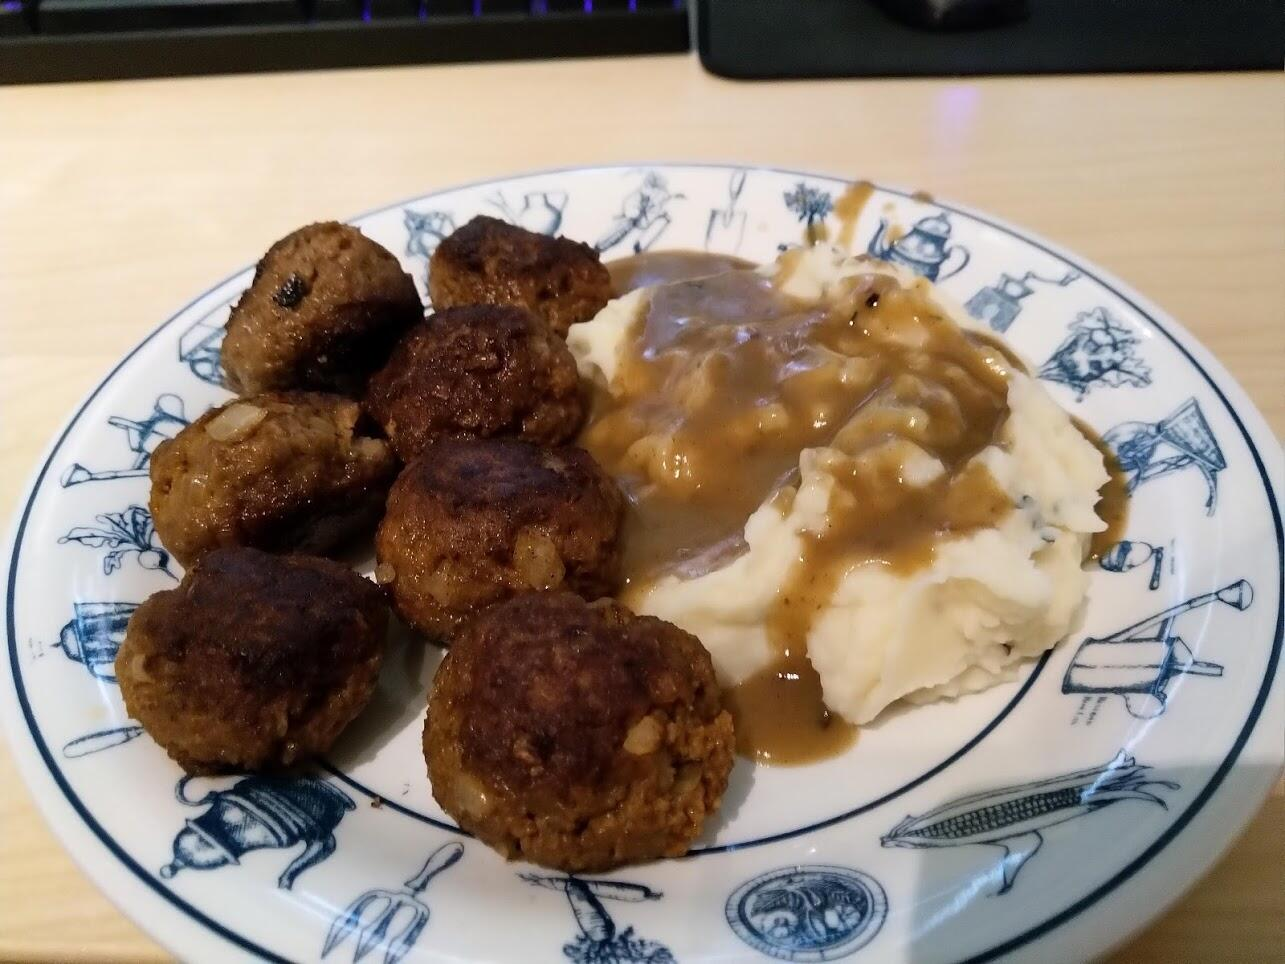
\includegraphics[height=\textheight]{meatballs/IMG_20190801_172405.jpg}}
	\end{figure}

    \introduction{
    	Alternatively, you can substitute \SI{1/2}{\pound} ground pork and \SI{1/2}{\pound} ground veal.

    	Serve with mashed potatoes.

    	Optionally, gravy.

    	Optionally, lingonberry jam.
	}

	\ingredients[13]{
		\SI{1/2}{\cup} & Milk \\
		\SI{1/2}{\cup} & Breadcrumbs \\
		1 & Yellow onion \\
		\SI{1}{\pound} & Ground beef (high fat content, get that good 20\% fat stuff if you can)  \\
		1 & Egg \\
		\SI{1}{\tablespoon} & Mustard (I usually use dijon, but you do you) \\
		\SI{2}{\tablespoon} & Paprika \\
		\SI{1}{\teaspoon} & Ground allspice \\
		& Salt (to taste) \\
		& Pepper (to taste) \\
		& Butter (for frying) \\
		& Vegetable oil (also for frying) \\
		& Cast-iron frying pan (guess what, for frying)
	}

	\preparation{

		\step In a bowl, mix milk and breadcrumbs until combined, then let sit.

		\step Chop the onion.

		\vspace{1em}

		\step Melt a bit of butter in the frying pan with some vegetable oil. Sweat the onion a bit in the pan, until translucent.

		\step Add onion and some of the fat to the bowl with the breadcrumb mixture. Add the ground meat, egg, mustard, and spices. Mix well.

		\step If brave, taste for seasoning and adjust accordingly.

		\step Lay out some parchment paper.

		\vspace{1em}

		\step With wet hands, roll meatball mixture into lots of small balls.

		\vspace{1em}

		\SIrange{1/2}{1}{\tablespoon} of mixture per ball is a good size.

		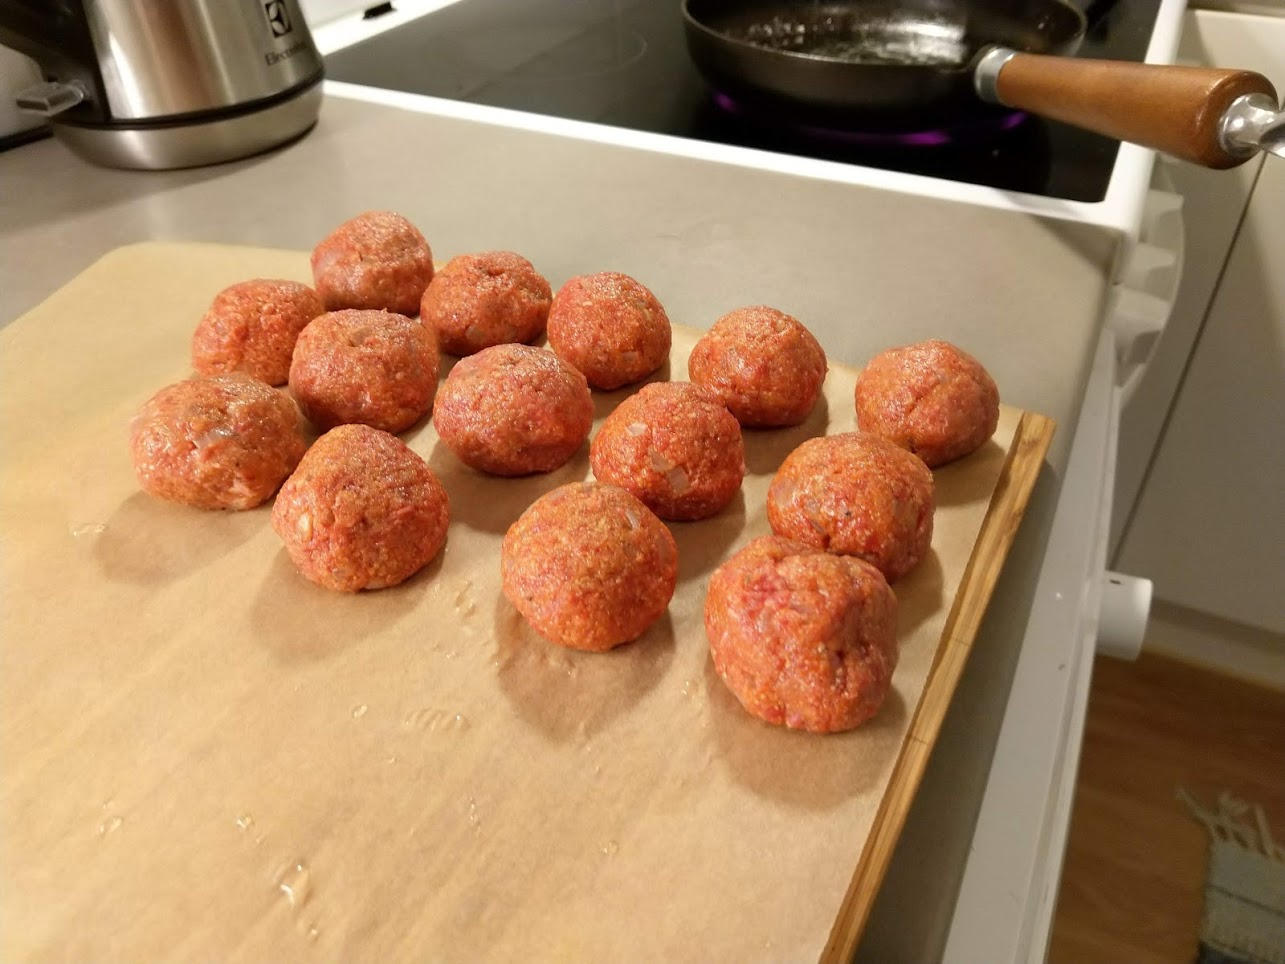
\includegraphics[width=\textwidth]{meatballs/IMG_20190801_165121.jpg}

		\step Get frying pan medium-hot, melt some more butter in it.

		\vspace{1em}

		\step Fry balls in batches for a few minutes per side, until nice and brown. Move balls into an oven-safe pan as you cook them. Keep the pan in a low oven as you cook the rest of the balls.
	}

\end{recipe}